% Compile with LuaLaTeX and BibTeX. See paper/README.md.
\documentclass[11pt]{article}

\usepackage[a4paper,margin=25mm,headheight=14pt]{geometry}
\usepackage{fontspec}
\defaultfontfeatures{Ligatures=TeX,Scale=MatchLowercase}
\setmainfont{Latin Modern Roman}
\setsansfont{Latin Modern Sans}
\setmonofont{Latin Modern Mono}
\usepackage{microtype}
\usepackage{setspace}
\usepackage{parskip}
\usepackage{amsmath,amssymb}
\usepackage{booktabs,tabularx,array}
\usepackage{graphicx}
\usepackage{caption,subcaption}
\usepackage[dvipsnames]{xcolor}
\usepackage{fancyhdr}
\usepackage[numbers,sort&compress]{natbib}
\usepackage{hyperref}

\definecolor{Ink}{HTML}{18212B}
\definecolor{Accent}{HTML}{176B87}
\definecolor{Rule}{HTML}{CBD5E1}
\definecolor{Link}{HTML}{0E7490}
\hypersetup{
  colorlinks=true,
  linkcolor=Accent,
  citecolor=Accent,
  urlcolor=Link,
  pdftitle={A Reproducible Comparison of Q-Learning, DQN, and PPO on Acrobot-v1},
  pdfauthor={Meet Mehta}
}
\urlstyle{same}
\graphicspath{{results/study/figures/}}
\captionsetup{font=small,labelfont={bf,color=Accent}}
\setstretch{1.05}
\setlength{\parindent}{0pt}
\setlength{\parskip}{5pt plus 1pt}
\setlength{\tabcolsep}{5pt}
\renewcommand{\arraystretch}{1.15}
\pagestyle{fancy}
\fancyhf{}
\lhead{Acrobot Reinforcement Learning Comparison}
\rhead{Meet Mehta}
\cfoot{\thepage}
\renewcommand{\headrulewidth}{0.4pt}
\fancypagestyle{plain}{
  \fancyhf{}
  \lhead{Acrobot Reinforcement Learning Comparison}
  \rhead{Meet Mehta}
  \cfoot{\thepage}
  \renewcommand{\headrulewidth}{0.4pt}
}

\newcommand{\method}[1]{\textsc{#1}}
\newcommand{\best}[1]{\textbf{#1}}
\newcommand{\code}[1]{\texttt{#1}}

\title{\vspace{-1.0cm}\textbf{A Reproducible Comparison of Q-Learning, DQN, and PPO on Acrobot-v1}}
\author{Meet Mehta\\\small Reinforcement Learning Project}
\date{August 2026}

\begin{document}
\maketitle

\begin{abstract}
This paper presents a reproducible comparison of tabular Q-Learning, Deep
Q-Networks (DQN), and Proximal Policy Optimization (PPO) on the underactuated
\code{Acrobot-v1} control task. All three algorithms were implemented from
scratch with NumPy and PyTorch; no prebuilt reinforcement-learning algorithm was
used. The protocol separates hyperparameter selection from final evaluation,
allocates an equal budget of 100,000 environment interactions to each method,
and evaluates deterministic policies every 5,000 interactions on ten fixed
held-out episodes. Final results aggregate five independent training seeds using
the interquartile mean (IQM) and bootstrap confidence intervals. Across this
budget, PPO was the only reliable solver, attaining a final held-out return IQM
of -81.7 (95\% CI: -87.5 to -74.4) and a 100\% success-rate IQM. DQN attained
-434.7 (95\% CI: -500.0 to -192.2) and displayed substantial seed sensitivity
and late-training regression. Discretized Q-Learning attained -480.5 (95\% CI:
-496.5 to -430.6) and did not cross the study's solved-return criterion on any
training seed. One-factor sensitivity experiments and component ablations further
show that DQN's target network and PPO's clipped objective materially improve
stability. The complete study contains 111 resumable runs, raw per-evaluation
episode data, configuration hashes, automated tests, and a self-contained Colab
demonstration.
\end{abstract}

\textbf{Keywords:} reinforcement learning; Acrobot; Q-Learning; Deep Q-Network;
Proximal Policy Optimization; reproducibility; robust evaluation

\section{Introduction}

Acrobot is a canonical nonlinear, underactuated control problem composed of two
links and a single actuator at their joint \citep{spong1995acrobot}. Because the
base joint is unactuated, a controller cannot lift the end effector directly. It
must instead coordinate torques to accumulate energy and swing the system above
a target height. This combination of continuous observations, sparse task
completion, and a small discrete action space makes Acrobot useful for comparing
representational and optimization choices in reinforcement learning (RL). The
benchmark's use in RL traces to sparse coarse-coding experiments by
\citet{sutton1995generalization}; the exact dynamics studied here are those in
Gymnasium 1.3.0.

This work compares three points on that design spectrum. Tabular Q-Learning is a
value-based baseline with a finite discretization of the observation space
\citep{watkins1992qlearning}. DQN replaces the table with a neural action-value
function and uses replay and a target network to stabilize bootstrapped learning
\citep{mnih2015human}. PPO is an on-policy actor-critic method that limits policy
changes through a clipped probability-ratio objective \citep{schulman2017ppo}.

RL comparisons can be unreliable when conclusions are drawn from a single seed,
training curves are mixed with evaluation results, or algorithms receive unequal
amounts of environment data \citep{henderson2018matters,agarwal2021precipice}.
Accordingly, this study emphasizes an auditable protocol rather than a leaderboard
number. Its contributions are:

\begin{itemize}
  \item from-scratch, tested implementations of Q-Learning, DQN, and PPO under one
        environment-interaction and evaluation harness;
  \item disjoint tuning and final seed sets, fixed held-out evaluation episodes,
        exact interaction budgets, and correct handling of termination versus
        time-limit truncation;
  \item robust multi-seed summaries, confidence intervals, sensitivity sweeps,
        and causal component ablations; and
  \item an openly inspectable artifact containing 111 raw runs, configuration
        files, generated plots, demonstration animations, and reproducibility
        instructions.
\end{itemize}

The central finding is conditional rather than universal: for the tested search
spaces and 100,000-interaction budget, PPO learned rapidly and consistently,
whereas DQN was unstable and the finite Q-table was not a reliable solver.

\section{Background and Related Work}

\subsection{Markov decision process}

An RL environment is modeled as a Markov decision process with state $s_t$,
action $a_t$, reward $r_t$, transition dynamics, and discount $\gamma$. A policy
$\pi(a\mid s)$ seeks to maximize expected discounted return
$G_t=\sum_{k=0}^{\infty}\gamma^k r_{t+k}$. The distinction between task
termination and an externally imposed time limit is important: a terminal state
has no future value, while a truncated trajectory may still bootstrap from its
last observation \citep{sutton2018reinforcement,towers2024gymnasium}.

\subsection{Tabular Q-Learning}

Q-Learning is an off-policy temporal-difference method that updates an action
value toward a greedy bootstrap target \citep{watkins1992qlearning}:
\begin{equation}
Q(s_t,a_t)\leftarrow Q(s_t,a_t)+\alpha
\left[r_t+\gamma(1-d_t)\max_a Q(s_{t+1},a)-Q(s_t,a_t)\right],
\label{eq:qlearning}
\end{equation}
where $d_t=1$ only for true task termination. Since Acrobot observations are
continuous, this implementation bins each dimension before indexing the table.
Discretization makes the method applicable but introduces aliasing: distinct
physical states can share one table entry.

\subsection{Deep Q-Network}

DQN approximates $Q(s,a)$ with parameters $\theta$ and minimizes a Huber loss
between the online prediction and a target
\begin{equation}
y_t=r_t+\gamma(1-d_t)\max_a Q(s_{t+1},a;\theta^-),
\label{eq:dqn}
\end{equation}
where $\theta^-$ denotes a periodically synchronized target network
\citep{mnih2015human}. A replay buffer reduces short-range sample correlation and
reuses past transitions. These mechanisms address important failure modes, but
neural bootstrapping can remain sensitive to initialization, exploration, and
hyperparameters.

\subsection{Proximal Policy Optimization}

PPO optimizes a stochastic policy using data sampled from the current policy. If
$r_t(\theta)=\pi_\theta(a_t\mid s_t)/\pi_{\theta_{\mathrm{old}}}(a_t\mid s_t)$,
the clipped surrogate is \citep{schulman2017ppo}
\begin{equation}
L^{\mathrm{clip}}(\theta)=\mathbb{E}_t\!\left[
\min\!\left(r_t(\theta)\hat A_t,
\operatorname{clip}(r_t(\theta),1-\epsilon,1+\epsilon)\hat A_t\right)
\right].
\label{eq:ppo}
\end{equation}
The critic supplies state-value estimates, and Generalized Advantage Estimation
(GAE) trades variance against bias through $\lambda$-weighted temporal-difference
residuals \citep{schulman2016gae}. The implementation also uses value loss,
advantage normalization, mini-batches, multiple optimization epochs, and gradient
clipping.

\subsection{Reliable evaluation}

Deep RL results can vary substantially across random seeds. Henderson et al.
demonstrated that implementation and reporting choices can change apparent
rankings \citep{henderson2018matters}. Agarwal et al. recommend performance
profiles, interval estimates, and robust aggregate statistics such as IQM rather
than relying only on point estimates from a few runs
\citep{agarwal2021precipice}. This study adopts IQM and bootstrap intervals while
also retaining every episode-level evaluation return. Unlike the multi-task
setting emphasized by Agarwal et al., the present IQM is computed across training
seeds for one task and the ordinary bootstrap resamples those seeds.

\section{Environment and Implementations}

\subsection{Acrobot-v1}

The Gymnasium environment exposes the six-dimensional observation
\begin{equation*}
[\cos\theta_1,\ \sin\theta_1,\ \cos\theta_2,\ \sin\theta_2,\
\ \dot\theta_1,\ \dot\theta_2]
\end{equation*}
and three discrete torque actions \citep{gymnasium_acrobot}. Each nonterminal step returns $-1$, so episode return
is the negative count of transitions before the successful terminal transition
(which returns zero); it therefore closely tracks episode length, and a
less-negative return is better. Episodes are capped at 500 steps. The project uses $-100$ as a
diagnostic solved-return threshold. This matches the environment's nominal reward
threshold, but the study checks it on ten fixed episodes at each evaluation rather
than claiming the separate 100-episode benchmark convention.

\subsection{Implementation details}

All algorithms were written in Python using NumPy for tabular and statistical
operations and PyTorch for neural networks \citep{harris2020numpy,paszke2019pytorch}.
No prebuilt RL training library was used. Q-Learning uses bins
$[8,8,8,8,10,10]$, learning rate $0.1$, discount $0.995$, and epsilon decay over
75,000 interactions. DQN uses two 128-unit hidden layers, learning rate
$3\times10^{-4}$, batch size 32, replay capacity 100,000, one update every four
steps after 1,000 warm-up steps, and target synchronization every 1,000 steps.
PPO uses two 64-unit hidden layers for its actor-critic network, learning rate
$10^{-3}$, $\gamma=0.99$, GAE $\lambda=0.95$, clip ratio $0.3$, 1,024-step
rollouts, ten optimization epochs, and mini-batches of 64. Equal-budget tuning
selected a zero entropy coefficient; consequently, entropy removal was not
reported as an ablation because it would be identical to the tuned control.

Python, NumPy, PyTorch, exploration generators, environment resets, and action
spaces are seeded. Research runs use one CPU thread per process to improve timing
comparability and parallel throughput. Saved records include the full resolved
configuration and a configuration-derived key, enabling completed runs to be
resumed without accidental duplication.

\section{Experimental Methodology}

\subsection{Study design}

The study has four groups totaling 111 runs:
\begin{itemize}
  \item \textbf{Tuning (54 runs):} six sampled configurations per method, each
        evaluated on three tuning-only seeds (100--102) for 25,000 interactions.
  \item \textbf{Final comparison (15 runs):} three methods, five disjoint training
        seeds (0--4), and 100,000 interactions per run.
  \item \textbf{Sensitivity (36 runs):} four values of one focal hyperparameter
        for each method, three seeds per value, and 50,000 interactions per run.
  \item \textbf{Ablation (6 runs):} DQN without a target network and PPO without
        clipping, each over three seeds and 50,000 interactions.
\end{itemize}

The tuner ranks candidates lexicographically by mean final held-out return, using
learning-curve area as a tie-breaker. The chosen configuration is fixed before
final-seed evaluation. Although
the sensitivity and ablation seeds overlap with final seeds 0--2, those diagnostic
experiments do not select the reported final configuration.

\subsection{Evaluation protocol}

Training is budgeted by environment interactions because episode count is partly
a consequence of policy quality. Every 5,000 training interactions, including at
step zero and the final step, the current policy is frozen and evaluated greedily
on ten environments reset with fixed held-out seeds 90,000--90,009. Evaluation
transitions never enter training data. Success is the fraction of episodes ending
through the environment's task-termination condition rather than time-limit
truncation.

For each final checkpoint, the study reports return and success IQM across five
training seeds. For sorted observations $x_{(1)},\ldots,x_{(n)}$, IQM is the mean
over the central 50\% of the empirical distribution, using fractional boundary
weights when needed. Final-return 95\% confidence intervals use 10,000 seeded
nonparametric bootstrap resamples of the five training seeds. Learning-curve bands
use the same estimator with 1,000 resamples per evaluation point. Because five
seeds remain a modest sample, intervals and per-seed plots are interpreted
together.

\section{Results}

\subsection{Learning performance}

\begin{figure}[htbp]
  \centering
  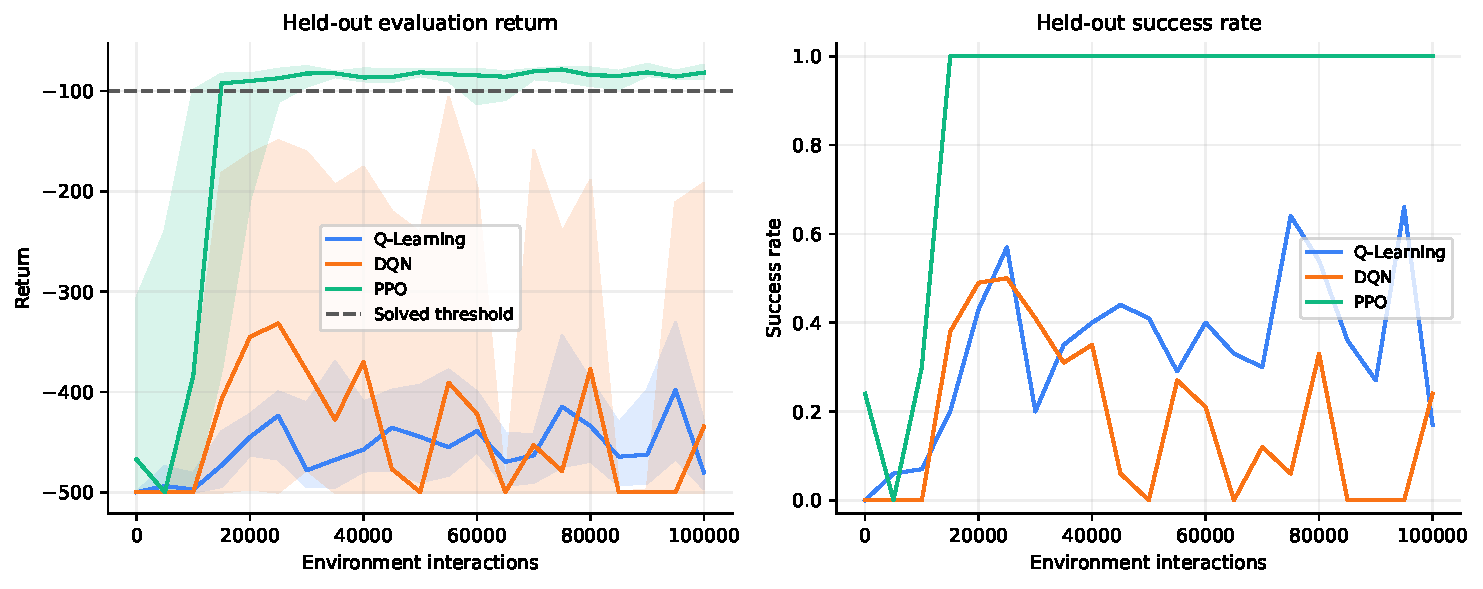
\includegraphics[width=\textwidth]{learning_curves.pdf}
  \caption{Held-out evaluation during training. Lines are the cross-seed IQM;
  the return panel's shaded regions are bootstrap intervals. The dashed line marks the study's
  $-100$ diagnostic threshold. PPO reaches high return and success reliably,
  whereas DQN and Q-Learning remain variable.}
  \label{fig:learning}
\end{figure}

Figure~\ref{fig:learning} shows a clear difference in both learning speed and
stability. PPO crosses the diagnostic threshold at a median of 15,000 interactions
and remains near a 100\% held-out success IQM. DQN improves on some seeds but its
aggregate return oscillates and degrades late in training. Q-Learning occasionally
terminates individual held-out episodes but never crosses the mean-return criterion
on any training seed.

\begin{table}[htbp]
\centering
\caption{Final held-out performance and computational measurements. Return is
the negative count of nonterminal transitions, so higher is better. CIs are 95\% bootstrap intervals
for final-return IQM. ``Never solved'' is based on periodic mean return.}
\label{tab:main}
\small
\begin{tabularx}{\textwidth}{>{\raggedright\arraybackslash}Xrrrrrr}
\toprule
Method & Seeds & Return IQM & 95\% CI & Success IQM & Median solve & Time (s) \\
\midrule
PPO & 5 & \best{-81.7} & $[-87.5,-74.4]$ & \best{100\%} & \best{15,000} & 30.5 \\
DQN & 5 & -434.7 & $[-500.0,-192.2]$ & 24\% & 65,000 & 18.8 \\
Q-Learning & 5 & -480.5 & $[-496.5,-430.6]$ & 17\% & Not reached & \best{6.6} \\
\bottomrule
\end{tabularx}
\end{table}

Table~\ref{tab:main} quantifies the gap. PPO's final interval lies entirely above
the $-100$ threshold. The wide DQN interval reflects markedly different outcomes:
its five final returns were $-424.4$, $-383.1$, $-500.0$, $-500.0$, and $-110.4$.
PPO's corresponding returns were tightly grouped from $-89.5$ to $-71.8$.
Q-Learning was computationally inexpensive but ended between $-500.0$ and
$-413.7$ across seeds.

\subsection{Seed stability}

\begin{figure}[htbp]
  \centering
  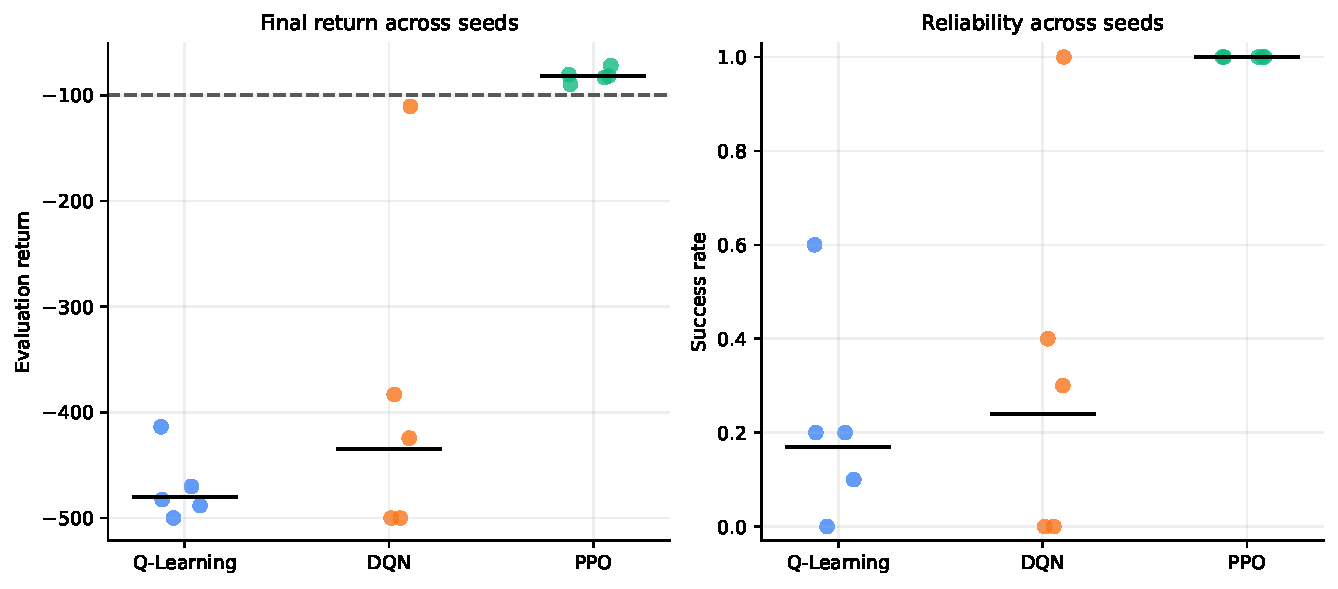
\includegraphics[width=0.94\textwidth]{seed_stability.pdf}
  \caption{Final return and success for each independent training seed. Horizontal
  black segments show the IQM. PPO is tightly clustered; DQN is seed-sensitive;
  Q-Learning remains close to the time limit.}
  \label{fig:seeds}
\end{figure}

The per-seed view in Figure~\ref{fig:seeds} prevents a best-run interpretation.
Four of five DQN seeds crossed $-100$ at least once during periodic evaluation,
but only one retained near-solved final performance. This difference between
``ever solved'' and ``final performance'' is evidence of policy regression, not a
contradiction. PPO reached the criterion on all seeds and retained final success.

\subsection{Hyperparameter sensitivity}

\begin{figure}[htbp]
  \centering
  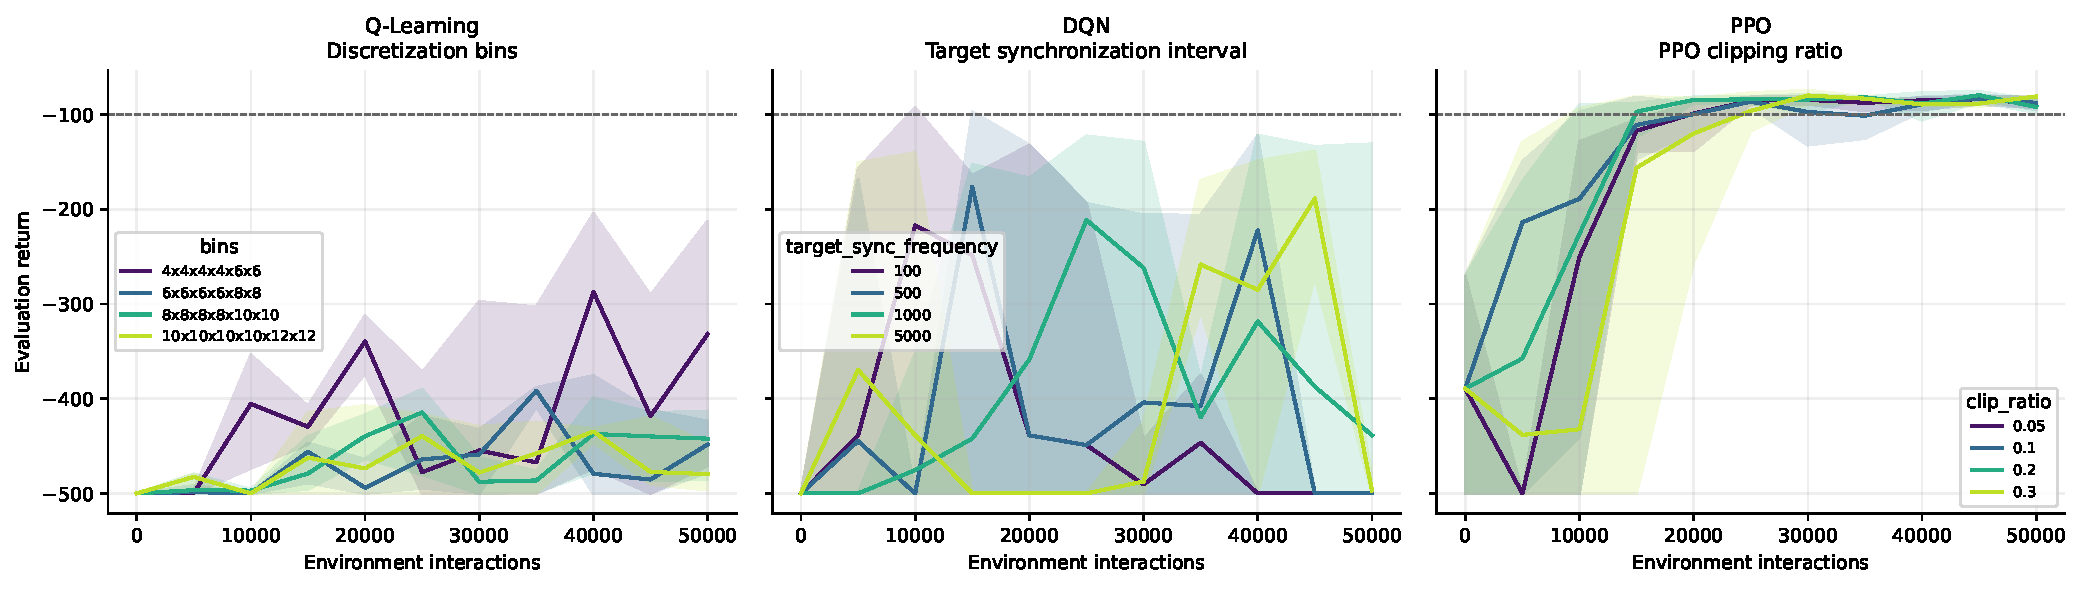
\includegraphics[width=\textwidth]{hyperparameter_sweeps.pdf}
  \caption{One-factor sensitivity studies at 50,000 interactions and three seeds
  per setting: Q-table discretization, DQN target synchronization interval, and
  PPO clipping ratio. Lines and bands are IQM and bootstrap intervals.}
  \label{fig:sweeps}
\end{figure}

Figure~\ref{fig:sweeps} indicates that the apparent ranking is not independent of
design choices. Q-Learning's table resolution changes both early generalization
and the number of state-action entries. DQN synchronization frequency produces
large, overlapping uncertainty bands, consistent with unstable value targets.
Across the examined PPO ratios, several settings eventually learn, but their
transient sample efficiency differs. These sweeps are diagnostic rather than an
exhaustive hyperparameter optimization.

\subsection{Component ablations}

\begin{figure}[htbp]
  \centering
  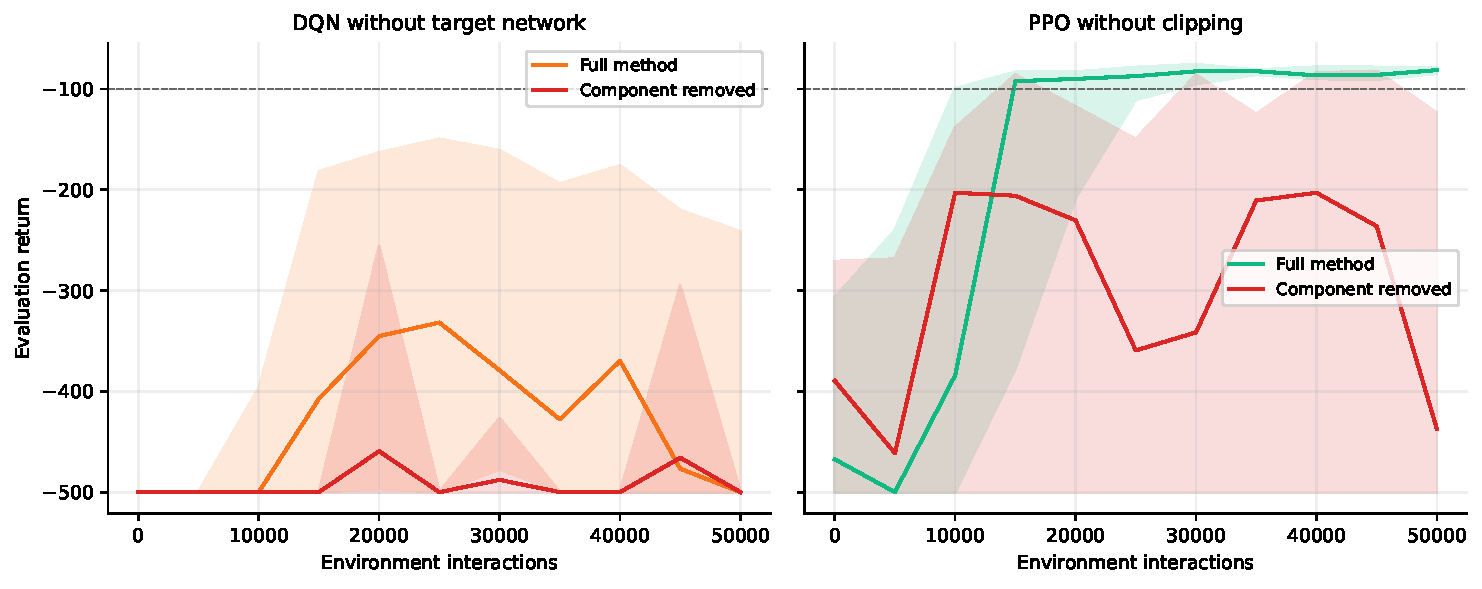
\includegraphics[width=\textwidth]{ablations.pdf}
  \caption{Component ablations over 50,000 interactions and three seeds. Removing
  DQN's target network prevents sustained learning; removing PPO clipping produces
  substantially worse and more variable performance.}
  \label{fig:ablations}
\end{figure}

The ablations in Figure~\ref{fig:ablations} test mechanisms rather than algorithm
labels. When DQN bootstraps from the rapidly changing online network, aggregate
performance remains at or near the 500-step limit. Unclipped PPO sometimes
improves, but repeatedly regresses and finishes far below the clipped control.
The experiments therefore support the stabilizing roles attributed to target
networks and clipped policy updates in Equations~\ref{eq:dqn} and~\ref{eq:ppo}.

\subsection{Computational efficiency}

\begin{figure}[htbp]
  \centering
  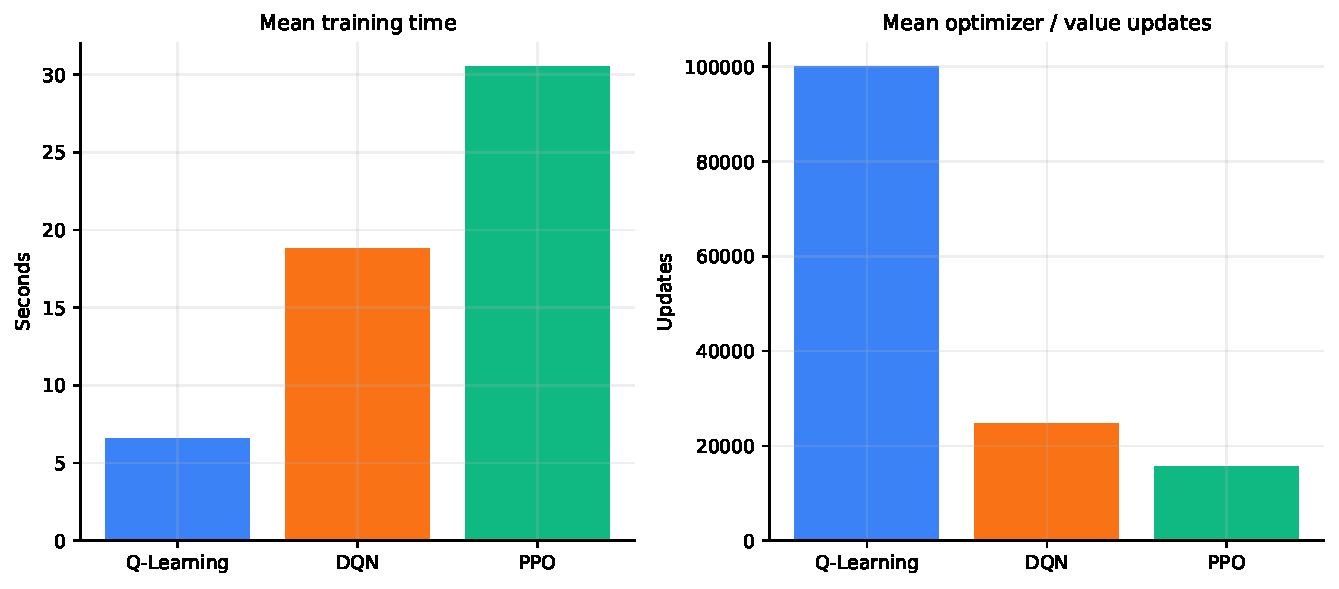
\includegraphics[width=0.92\textwidth]{computational_efficiency.pdf}
  \caption{Mean local CPU training time and mean update count for 100,000
  interactions. Wall-clock values characterize this machine and implementation;
  they are not hardware-independent complexity measurements.}
  \label{fig:efficiency}
\end{figure}

Q-Learning is fastest at 6.6 seconds per seed but performs 100,000 direct table
updates. DQN averages 18.8 seconds and 24,751 optimizer updates because it learns
every fourth step after replay warm-up. PPO averages 30.5 seconds and 15,630
mini-batch optimizer updates. Figure~\ref{fig:efficiency} shows that fewer optimizer
updates need not imply lower wall-clock time: PPO performs multiple epochs over
rollouts and evaluates both actor and critic losses.

\section{Discussion}

PPO's advantage in this experiment is primarily a reliability result. Its policy
objective updates action probabilities directly, its critic reduces gradient
variance, and clipping limits harmful changes to the data-collecting policy. The
method consistently transformed the same interaction budget into successful
swing-up behavior. The ablation provides within-method evidence that clipping is
important under the selected configuration.

DQN's mixed outcomes are equally informative. Function approximation avoids the
explicit state aliasing of a Q-table, yet bootstrapping and off-policy replay create
a moving optimization problem. The target-network ablation shows an extreme form
of that instability. Even with the target network, the divergence between
intermediate and final evaluations suggests that a future study should preregister
a checkpoint-selection rule using tuning seeds rather than assume that the last
network is best.

Q-Learning demonstrates a computational-versus-statistical trade-off. Its update
is simple and fast, but the selected table contains
$8^4\times10^2\times3=1{,}228{,}800$ entries. Many entries receive limited data,
while binning also aliases states near a boundary. Coarser bins generalize more
aggressively but lose precision; finer bins require more experience. Tile coding
or radial basis functions could improve representation, but would constitute a
different baseline.

The results should not be read as proof that PPO universally dominates DQN or
Q-Learning. They establish a reproducible conditional claim: with these
implementations, equal tuning budgets, search spaces, and 100,000 Acrobot
interactions, PPO was more sample-efficient and reliable.

\section{Threats to Validity and Limitations}

\textbf{Statistical power.} Five final training seeds are stronger than a single
run but still permit wide uncertainty, especially for DQN. Bootstrap intervals do
not manufacture information absent from the sample.

\textbf{Evaluation set size.} Each periodic point uses ten fixed held-out episodes.
This supports controlled comparisons and exposes episode-level outcomes, but it
is smaller than the environment's conventional 100-episode threshold procedure.

\textbf{Search-space dependence.} Equal trial counts create procedural fairness,
not a guarantee that each algorithm's globally best configuration was found. A
broader or adaptive search could change performance.

\textbf{Single environment.} Acrobot has discrete actions and particular dynamics.
Generalization to continuous-action control, image observations, or other reward
structures is untested.

\textbf{Shared diagnostic seeds.} Sensitivity and ablation experiments use seeds
0--2, which overlap the final training seeds. They are interpreted only as
mechanistic diagnostics and do not alter the final chosen hyperparameters.

\textbf{Timing.} Wall-clock results come from local CPU execution with small
networks. They should not be extrapolated to accelerators or other hardware.

\section{Reproducibility and Artifact}

The artifact stores each run as JSON plus a CSV containing evaluation step, mean
return, success rate, and the ten episode returns. YAML files define the study and
selected parameters. Matching runs are identified by a hash of the complete run
specification and skipped on resume. Plot and table scripts read raw records; no
benchmark values are hard-coded into analysis code. The repository also includes
unit and integration tests for discretization, Bellman targets, replay sampling,
target synchronization, GAE, PPO clipping, termination handling, ablation switches,
statistics, and persistence. Fourteen tests pass in the verified environment.

The complete study can be regenerated with:
\begin{verbatim}
uv sync --locked --extra dev
uv run pytest -q
uv run python run_study.py --workers 4 all
\end{verbatim}
The generated plots are available in both PNG and vector PDF formats, while saved
checkpoints can be rendered as GIFs or in a live Gymnasium window. A standalone
13-cell Colab notebook provides a lower-cost classroom demonstration.

\section{Conclusion}

This study compared tabular Q-Learning, DQN, and PPO on Acrobot using a common,
equal-interaction protocol and robust multi-seed reporting. PPO achieved reliable
solution behavior within 100,000 interactions, with final return IQM $-81.7$ and
100\% success IQM. DQN learned on several seeds but frequently regressed, while
Q-Learning's discretized representation was fast but unreliable at this budget.
Sensitivity plots and ablations showed that conclusions depend on important design
choices and supported the stabilizing roles of DQN's target network and PPO's
clipped objective. More broadly, the work illustrates that reproducible RL
comparison requires separating tuning from evaluation, controlling data budgets,
retaining per-seed evidence, and reporting uncertainty rather than presenting a
single successful trajectory.

\section*{Data and Code Availability}

The code, configurations, raw experimental records, generated figures, tables,
tests, and Colab notebook are included with the project repository. A public URL
will be added after the repository is pushed to GitHub.

\bibliographystyle{plainnat}
\bibliography{paper/references}

\appendix
\section{Selected Hyperparameters}

\begin{table}[htbp]
\centering
\caption{Hyperparameters selected using tuning seeds 100--102. Parameters not
listed here retain the implementation defaults described in Section 3.}
\label{tab:hyperparameters}
\small
\begin{tabularx}{\textwidth}{>{\bfseries}lX}
\toprule
Method & Selected parameters \\
\midrule
Q-Learning & learning rate $0.1$; discount $0.995$; epsilon decay 75,000;
bins $[8,8,8,8,10,10]$ \\
DQN & learning rate $3\times10^{-4}$; batch size 32; target synchronization
1,000; epsilon decay 50,000 \\
PPO & learning rate $10^{-3}$; clip ratio $0.3$; rollout 1,024; entropy
coefficient $0.0$ \\
\bottomrule
\end{tabularx}
\end{table}

\clearpage
\section{Per-Seed Final Results}

\begin{center}
\captionsetup{hypcap=false}
\captionof{table}{Final held-out return and success rate for every final training seed.}
\label{tab:perseed}
\centering
\small
\begin{tabular}{llrrr}
\toprule
Method & Seed & Return & Success & First threshold crossing \\
\midrule
Q-Learning & 0 & -470.0 & 20\% & Not reached \\
Q-Learning & 1 & -500.0 & 0\% & Not reached \\
Q-Learning & 2 & -482.5 & 20\% & Not reached \\
Q-Learning & 3 & -413.7 & 60\% & Not reached \\
Q-Learning & 4 & -488.3 & 10\% & Not reached \\
\midrule
DQN & 0 & -424.4 & 30\% & Not reached \\
DQN & 1 & -383.1 & 40\% & 95,000 \\
DQN & 2 & -500.0 & 0\% & 70,000 \\
DQN & 3 & -500.0 & 0\% & 55,000 \\
DQN & 4 & -110.4 & 100\% & 60,000 \\
\midrule
PPO & 0 & -81.8 & 100\% & 30,000 \\
PPO & 1 & -80.4 & 100\% & 15,000 \\
PPO & 2 & -71.8 & 100\% & 10,000 \\
PPO & 3 & -89.5 & 100\% & 15,000 \\
PPO & 4 & -83.0 & 100\% & 15,000 \\
\bottomrule
\end{tabular}
\end{center}

\end{document}
